\section{A neural operator informed by a ROM}\label{sec:vf-frino}

\subsection*{Concept and purpose}

\citet{yang2025frino} train a Fourier neural operator (FNO) to map an excitation history to the structural response, and add to the data loss a term that penalises the residual of a low-order POD Galerkin ROM of the same structure. The ROM supplies the physics at the cost of a few reduced equations, the finite element model supplies the training labels, and the trained operator is meant to predict responses to new waveforms in milliseconds. The study rebuilds the pipeline end to end (a three-dimensional finite element cantilever, its POD ROM, the operator, the publication's test loads and parameter studies) and adds checks the publication omits: whether the operator is linear, how much the physics term contributes, how strong a tuned PINN baseline is, and what the exact frequency-domain solution of this linear problem costs.

The packages supply the finite element model (\anchor{fea_engine.elements.Hex20}), the POD ROM and the Newmark integrators of \rom{}, the exact frequency-domain solve (paper Eq.~20) and, for double precision, the FNO blocks of \rom{}; the network training itself used PyTorch on a 3~GB GPU in single precision.

\subsection*{Mathematics as implemented}

The full-order model is $\mathbf M\ddot{\mathbf u}+\mathbf C\dot{\mathbf u}+\mathbf K\mathbf u=\mathbf f\,g(t)$ with Rayleigh damping $\mathbf C=0.154\,\mathbf M+0.00078\,\mathbf K$. A POD basis $\boldsymbol\Psi$ of three modes is built from 200 snapshots of the single-tone responses, $\mathbf u\approx\boldsymbol\Psi\mathbf q$, giving the ROM
\begin{equation}\label{eq:fr-rom}
\mathbf M_r\ddot{\mathbf q}+\mathbf C_r\dot{\mathbf q}+\mathbf K_r\mathbf q=\boldsymbol\Psi^{T}\mathbf f\,g(t).
\end{equation}
The operator maps the excitation $g$ on the time grid to the reduced coordinates $\mathbf q$, and is trained on
\begin{equation}\label{eq:fr-loss}
\mathcal L=\mathcal L_{\rm data}+\lambda\,\mathcal L_{\rm ROM},\qquad
\mathcal L_{\rm ROM}=\big\lVert\mathbf M_r\ddot{\mathbf q}_\theta+\mathbf C_r\dot{\mathbf q}_\theta+\mathbf K_r\mathbf q_\theta-\boldsymbol\Psi^{T}\mathbf f\,g\big\rVert^2,
\end{equation}
with the time derivatives of the network output formed by finite differences on the time grid; the data loss is on the labels of the ROM time stepping at the training points. All errors are relative $L_2$ against the 4239-degree-of-freedom response unless stated, evaluated through the projection identity
\begin{equation}\label{eq:fr-err}
\lVert\mathbf u-\boldsymbol\Psi\mathbf q\rVert^2=\lVert\mathbf u\rVert^2-2\langle\boldsymbol\Psi^{T}\mathbf u,\mathbf q\rangle+\lVert\mathbf q\rVert^2,
\end{equation}
which gives full-field errors without storing the full-order fields. Because the ROM is linear and time-invariant, its response to a harmonic load follows from a frequency-domain solve of \cref{eq:fr-rom} (the publication's Eq.~20), exact up to the discretisation of the transform; this is the baseline against which the operator's cost is compared. A forced--transient split of the ROM response is used to interpret the high-frequency errors.

\subsection*{Geometry and mesh}

The structure is the cantilever of the publication, $60\times15\times1.5$~mm, with a point load at the midpoint of the free end, transverse to the thickness (\Cref{fig:vf-fr-geom}). The publication used an ANSYS Solid186 model with 4239 degrees of freedom; the analogue here is a $14\times8\times2$ mesh of twenty-node hexahedra, with 1413 nodes, 4239 degrees of freedom and 4032 free ones. Material constants are printed in a garbled unit string in the publication; they are used as printed ($E=2\times10^5$~N/mm$^2$, $\rho=7.9\times10^{-6}$), which gives $f_1=10.9$~Hz against the publication's 10~Hz, and the consistent-unit alternative gives 345~Hz. \Cref{tab:vf-fr-setup} lists what the publication states and what was chosen.

\begin{figure}[tbp]
\centering
\includegraphics[width=0.9\linewidth]{figures/ch14_geom_frino.pdf}
\caption{Cantilever of the neural-operator study, drawn from the data of the report: $14\times8\times2$ Hex20 elements, clamped end and the transverse point load at the free end.}\label{fig:vf-fr-geom}
\end{figure}

\begin{table}[tbp]
\centering\footnotesize
\caption{Set-up of the neural-operator study.}\label{tab:vf-fr-setup}
\begin{tabularx}{\linewidth}{@{}>{\raggedright\arraybackslash}p{2.6cm} >{\raggedright\arraybackslash}X >{\raggedright\arraybackslash}X@{}}
\toprule
Item & Publication & This work\\
\midrule
Geometry & $60\times15\times1.5$ mm cantilever, point load at free-end midpoint & same; load transverse to the thickness\\
Model & ANSYS Solid186, 4239 dofs & \texttt{Hex20}, $14\times8\times2$, 4239 dofs (4032 free)\\
Material & $E$, $\rho$ in a garbled unit string & $E=2\times10^5$ N/mm$^2$, $\rho=7.9\times10^{-6}$ as printed ($f_1=10.9$ Hz)\\
Damping & $\mathbf C=0.154\,\mathbf M+0.00078\,\mathbf K$ & same\\
Time window & 0.41 s, 8192 points, 6.25\,\% (512 points) for training & same\\
POD & 200 snapshots, 3 modes & 200 snapshots from the 8 single-tone responses (which response is not stated), 3 modes\\
FNO & 4 Fourier layers, width 256 & same; 64 Fourier modes (not stated); time-grid channel appended\\
Training & 500 epochs, batch 20, Adam lr $10^{-3}$, $\times0.4$ every 100 epochs, $\lambda=10^{-3}$ & same; weight decay $10^{-4}$\\
Training set & not stated & 8 paper tones + 32 random single tones in 2--120 Hz (40)\\
Loss scaling & raw & data loss on normalised modes; ROM residual normalised by the mean-square reduced load\\
Equations 35--36 & ``501 Hz'', ``701 Hz'' & read as 50 Hz, 70 Hz\\
Precision & --- & single (double supported with \rom{}'s own FNO blocks)\\
\bottomrule
\end{tabularx}
\end{table}

\subsection*{Results: full-order model, POD and ROM}

The first natural frequencies of the model are $10.9$, $68.2$, $85.0$, $102.9$ and $191.2$~Hz. The POD cumulative energy is $99.9871$, $99.99970$ and $100.00000\,\%$ for one, two and three modes against $94.610$, $99.954$ and $99.999\,\%$ in the publication, a difference that follows from the snapshot source, which the publication does not state. The three-mode ROM has eigenfrequencies $10.9$, $68.2$ and $227.8$~Hz and Rayleigh damping ratios $0.028$, $0.167$ and $0.558$. Solver cross-checks agree: GPU batched Newmark against CPU SuperLU Newmark on the tip degree of freedom to $5.9\times10^{-9}$, the study's beam integrator against \fea{}'s implicit transient to $10^{-9}$ (a unit test), and the GPU stiffness assembly against the loop assembly to $4\times10^{-15}$. \Cref{tab:vf-fr-ref} and \Cref{fig:vf-fr-fom} give the validation per load.

\begin{table}[tbp]
\centering\footnotesize
\caption{Reference-solver validation (three-mode ROM).}\label{tab:vf-fr-ref}
\begin{tabular}{@{}lrrr@{}}
\toprule
Load & POD truncation & 3-mode ROM against FEM & Eq.~(20) FFT solve against ROM stepping\\
\midrule
5 Hz & $4.924\times10^{-5}$ & $7.350\times10^{-5}$ & $3.781\times10^{-6}$\\
10 Hz & $1.016\times10^{-5}$ & $1.519\times10^{-5}$ & $1.224\times10^{-5}$\\
15 Hz & $4.653\times10^{-5}$ & $6.949\times10^{-5}$ & $8.112\times10^{-6}$\\
20 Hz & $9.246\times10^{-5}$ & $1.382\times10^{-4}$ & $9.140\times10^{-6}$\\
95 Hz & $1.466\times10^{-3}$ & $2.425\times10^{-3}$ & $8.301\times10^{-5}$\\
100 Hz & $1.738\times10^{-3}$ & $2.891\times10^{-3}$ & $7.795\times10^{-5}$\\
105 Hz & $2.085\times10^{-3}$ & $3.493\times10^{-3}$ & $7.448\times10^{-5}$\\
110 Hz & $2.499\times10^{-3}$ & $4.219\times10^{-3}$ & $7.213\times10^{-5}$\\
Fm1 & $1.977\times10^{-4}$ & $3.168\times10^{-4}$ & $1.774\times10^{-5}$\\
Fm2 & $6.252\times10^{-4}$ & $1.084\times10^{-3}$ & $4.036\times10^{-5}$\\
Fr1 & $1.745\times10^{-4}$ & $2.833\times10^{-4}$ & $1.732\times10^{-5}$\\
Fr2 & $1.374\times10^{-4}$ & $2.234\times10^{-4}$ & $1.743\times10^{-5}$\\
\bottomrule
\end{tabular}
\end{table}

\begin{figure}[tbp]
\centering
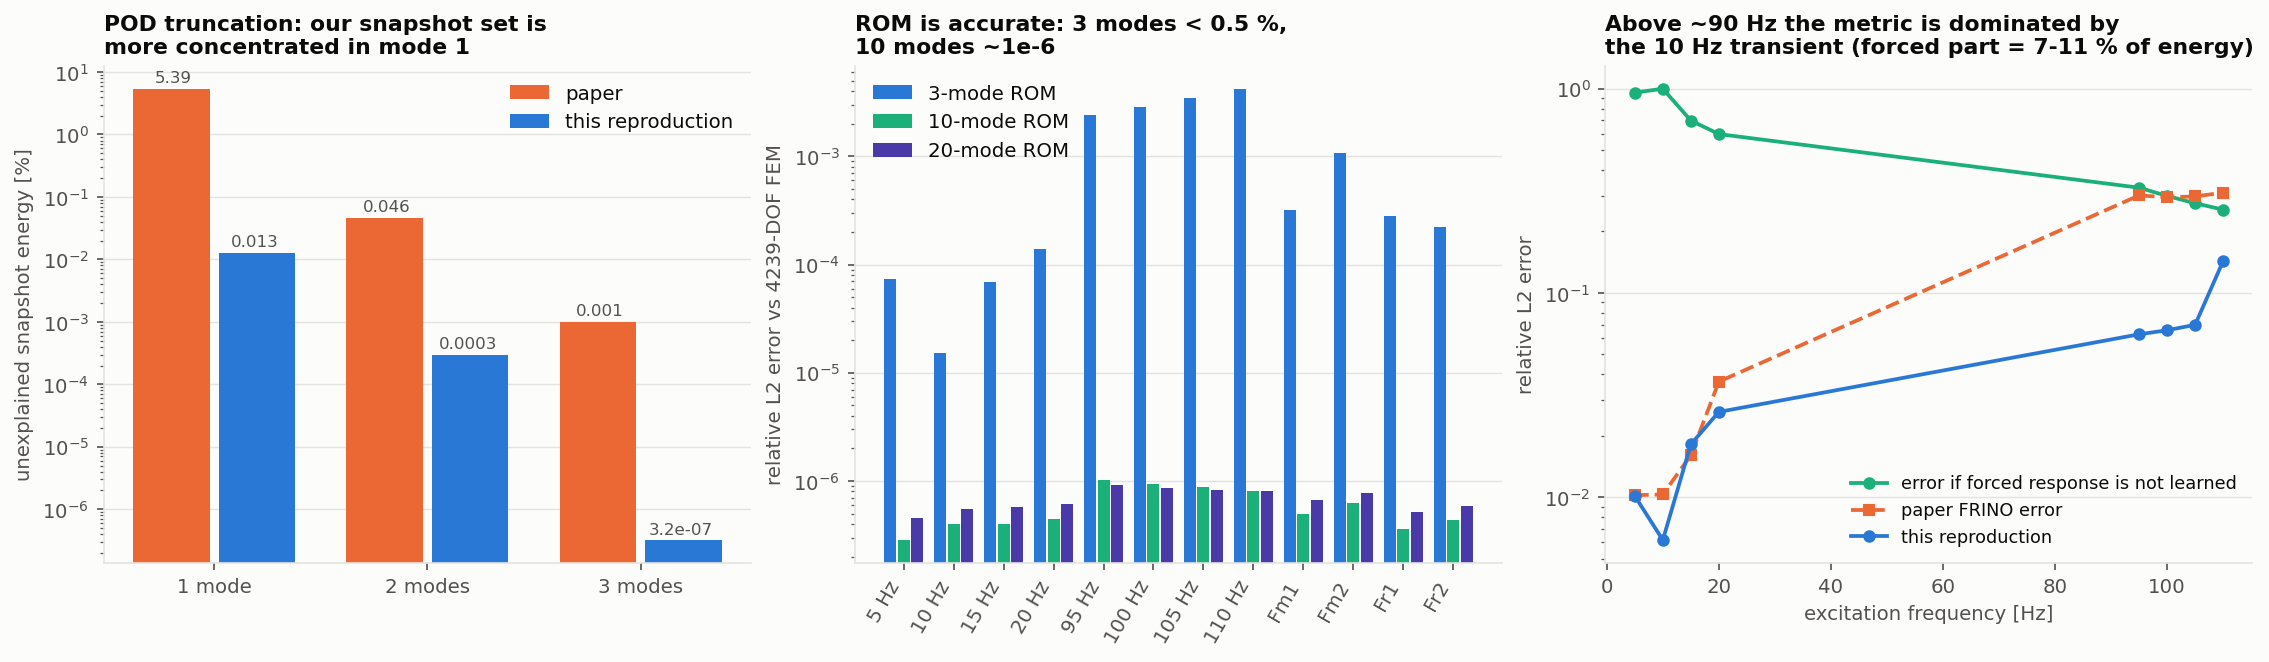
\includegraphics[width=0.98\linewidth]{figures/ch14r/fr_fom.png}
\caption{(a) Unexplained snapshot energy after 1--3 POD modes, publication against this work. (b) Relative error of the 3-, 10- and 20-mode ROM against the 4239-dof model for all 12 loads. (c) Error floor if the forced response is not learned, against the publication's and this work's single-tone errors. Plot of the reproduction report.}\label{fig:vf-fr-fom}
\end{figure}

\subsection*{Results: the operator on the publication's loads}

The default run has 33.9 million parameters, trains in 139~s and is evaluated on all 12 loads (eight single tones at 5, 10, 15, 20, 95, 100, 105 and 110~Hz, two multi-frequency loads Fm1, Fm2 and two random loads Fr1, Fr2). \Cref{tab:vf-fr-err} and \Cref{fig:vf-fr-err} compare with the publication. Single tones reproduce, with a mean of $1.5\times10^{-2}$ at 5--20~Hz (publication $1.8\times10^{-2}$) and $8.5\times10^{-2}$ at 95--110~Hz (publication $0.3$); the multi-frequency and random loads do not. The errors on the training grid and on a grid sixteen times finer agree to within a factor of two, and the errors against the ROM labels and against the finite element model agree to three digits, so POD truncation is not what limits accuracy.

\begin{table}[tbp]
\centering\footnotesize
\caption{Relative $L_2$ error against the 4239-dof FEM.}\label{tab:vf-fr-err}
\begin{tabular}{@{}lrrrr@{}}
\toprule
Load & Publication & This work, training grid & This work, 16$\times$ finer grid & Against ROM (finer grid)\\
\midrule
5 Hz & $1.02\times10^{-2}$ & $9.46\times10^{-3}$ & $1.01\times10^{-2}$ & $1.01\times10^{-2}$\\
10 Hz & $1.03\times10^{-2}$ & $4.76\times10^{-3}$ & $6.17\times10^{-3}$ & $6.17\times10^{-3}$\\
15 Hz & $1.60\times10^{-2}$ & $1.70\times10^{-2}$ & $1.81\times10^{-2}$ & $1.81\times10^{-2}$\\
20 Hz & $3.68\times10^{-2}$ & $2.61\times10^{-2}$ & $2.62\times10^{-2}$ & $2.62\times10^{-2}$\\
95 Hz & $3.00\times10^{-1}$ & $6.38\times10^{-2}$ & $6.27\times10^{-2}$ & $6.27\times10^{-2}$\\
100 Hz & $2.94\times10^{-1}$ & $6.95\times10^{-2}$ & $6.57\times10^{-2}$ & $6.56\times10^{-2}$\\
105 Hz & $2.97\times10^{-1}$ & $7.67\times10^{-2}$ & $6.98\times10^{-2}$ & $6.97\times10^{-2}$\\
110 Hz & $3.10\times10^{-1}$ & $9.92\times10^{-2}$ & $1.43\times10^{-1}$ & $1.43\times10^{-1}$\\
Fm1 & $1.29\times10^{-1}$ & $4.12\times10^{-1}$ & $4.07\times10^{-1}$ & $4.07\times10^{-1}$\\
Fm2 & $2.02\times10^{-1}$ & $5.36\times10^{-1}$ & $4.80\times10^{-1}$ & $4.80\times10^{-1}$\\
Fr1 & $9.65\times10^{-2}$ & $7.74\times10^{-1}$ & $7.74\times10^{-1}$ & $7.74\times10^{-1}$\\
Fr2 & $9.87\times10^{-2}$ & $6.09\times10^{-1}$ & $6.08\times10^{-1}$ & $6.08\times10^{-1}$\\
\bottomrule
\end{tabular}
\end{table}

\begin{figure}[tbp]
\centering
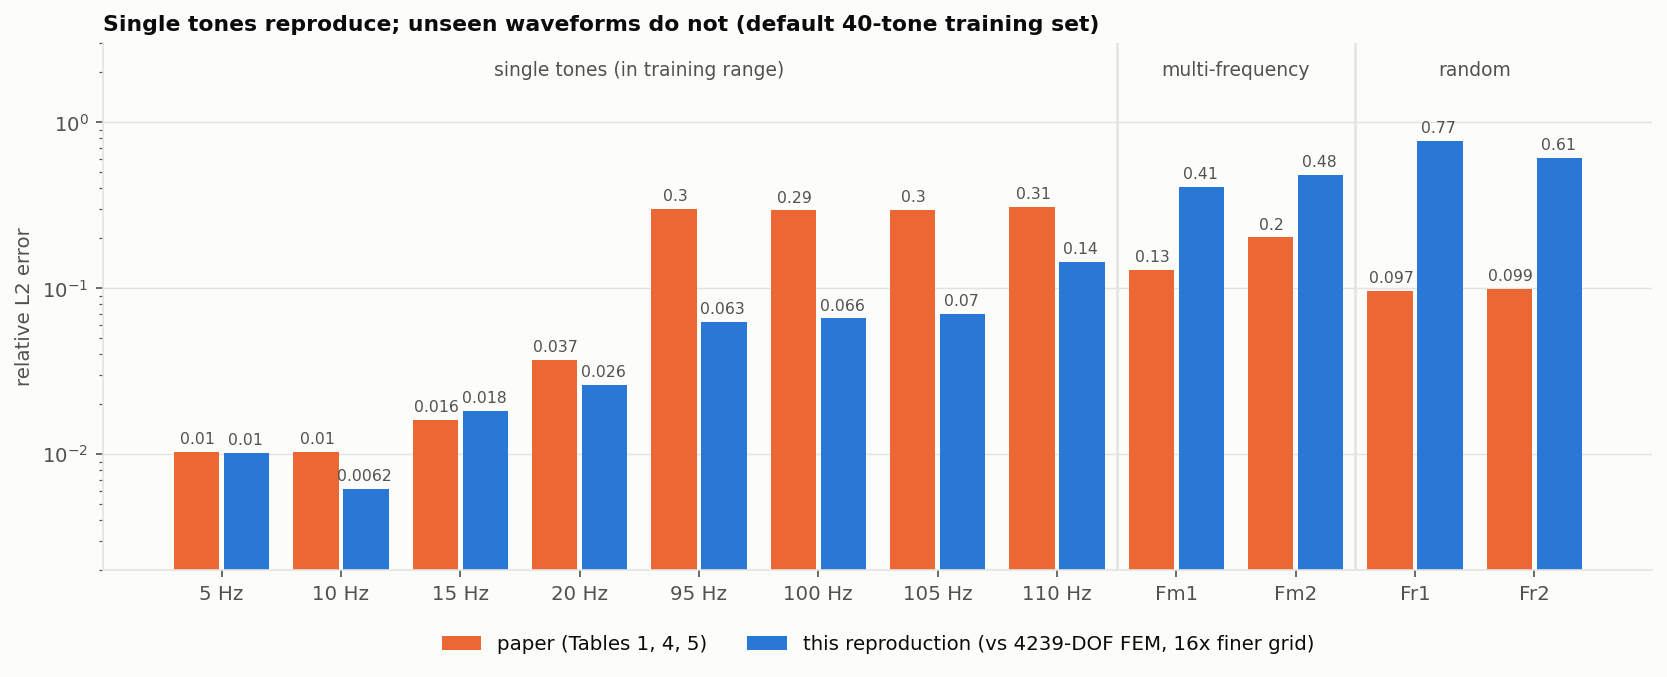
\includegraphics[width=0.9\linewidth]{figures/ch14r/fr_err.png}
\caption{Relative $L_2$ error for the 12 test loads: publication (Tables 1, 4, 5) against this work. Plot of the reproduction report.}\label{fig:vf-fr-err}
\end{figure}

\begin{figure}[tbp]
\centering
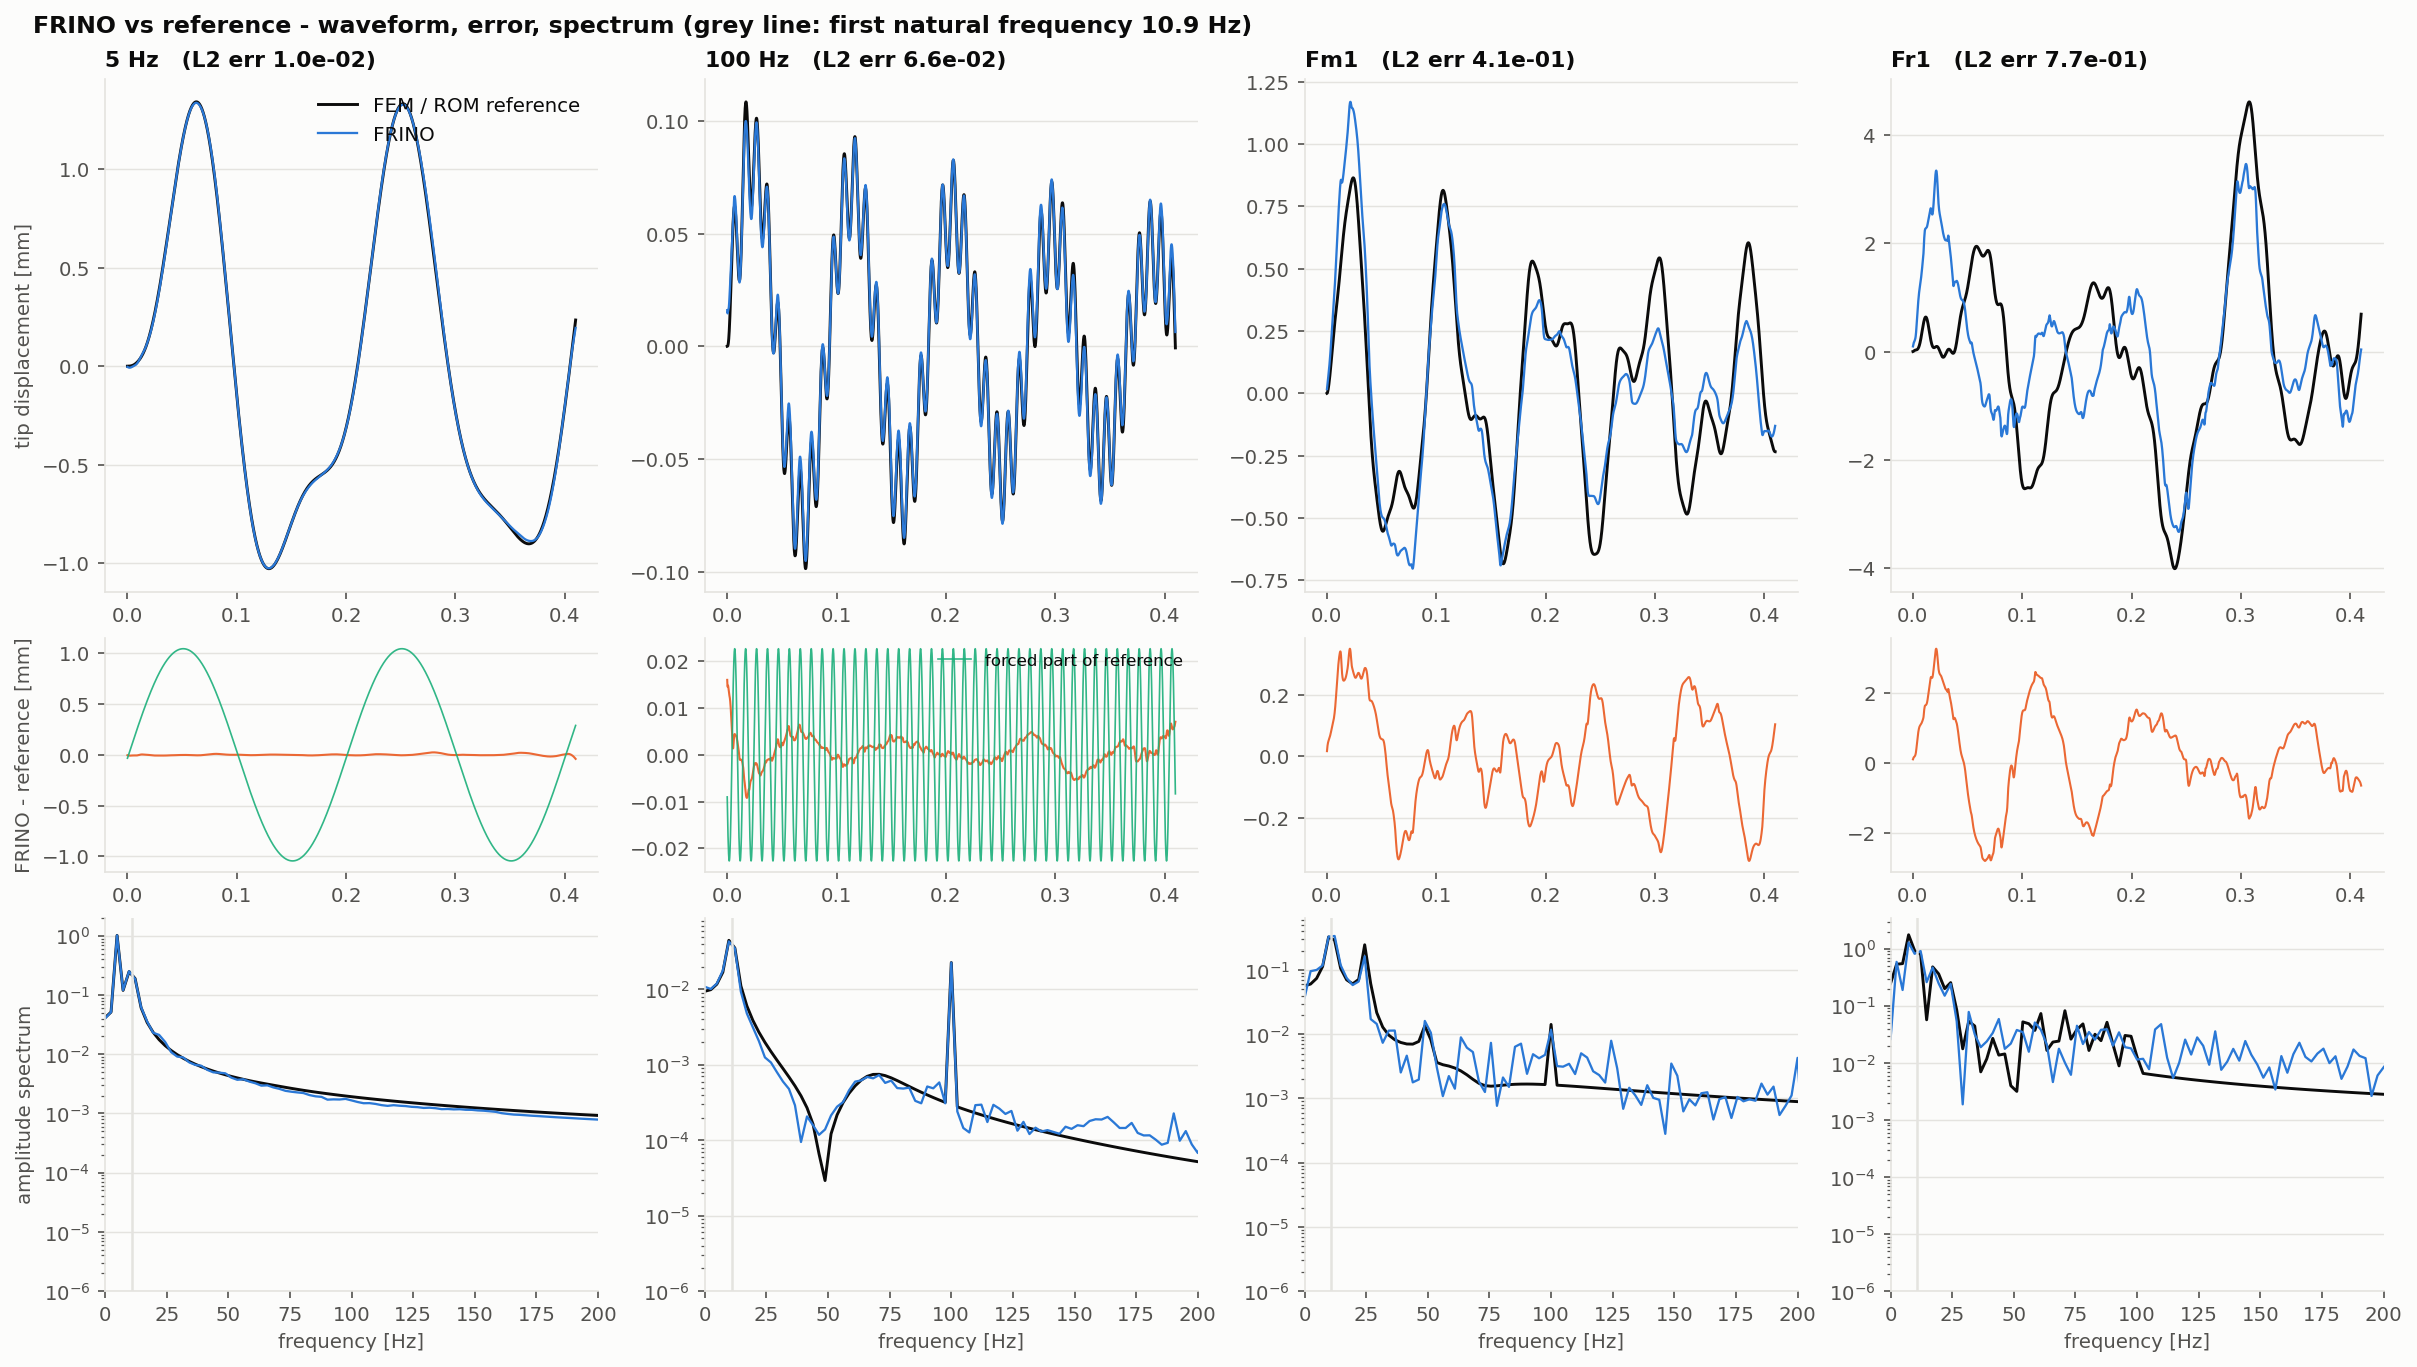
\includegraphics[width=0.98\linewidth]{figures/ch14r/fr_resp.png}
\caption{Tip displacement, operator-minus-reference error and amplitude spectrum for 5~Hz, 100~Hz, Fm1 and Fr1. At 5 and 100~Hz the waveforms are nearly indistinguishable and the 100~Hz forced peak is reproduced in the spectrum; on Fm1 and Fr1 the early-time peaks are missed. Plot of the reproduction report.}\label{fig:vf-fr-resp}
\end{figure}

\emph{Why the high-frequency error looks large in the publication.} \Cref{tab:vf-fr-forced} splits the ROM response into forced and transient parts. Above about 90~Hz the forced response carries only $7$--$11\,\%$ of the energy, because the 10~Hz free-decay transient dominates the $L_2$ norm; a model that missed the forced part entirely would show $0.26$--$0.33$, exactly the publication's $0.29$--$0.31$. The network here reproduces the forced peak at the excitation frequency to $0.46\,\%$ at all eight tones. The publication's high-frequency errors are therefore consistent with a network that has not learned the forced response, and a whole-window $L_2$ norm hides this.

\begin{table}[tbp]
\centering\footnotesize
\setlength{\tabcolsep}{3pt}
\caption{Forced against transient split of the 3-mode ROM response.}\label{tab:vf-fr-forced}
\begin{tabular}{@{}lrrrrrr@{}}
\toprule
Tone & Forced energy fraction & Floor if forced part missed & Error & Error / forced norm & Spectral-peak error at $f_{\rm exc}$ & Error above 40 Hz\\
\midrule
5 Hz & 0.918 & 0.958 & $1.01\times10^{-2}$ & $1.06\times10^{-2}$ & $3.1\times10^{-4}$ & ---\\
10 Hz & 1.154 & 1.000 & $6.17\times10^{-3}$ & $5.74\times10^{-3}$ & $5.2\times10^{-4}$ & ---\\
15 Hz & 0.488 & 0.699 & $1.81\times10^{-2}$ & $2.60\times10^{-2}$ & $1.1\times10^{-3}$ & ---\\
20 Hz & 0.360 & 0.600 & $2.62\times10^{-2}$ & $4.36\times10^{-2}$ & $1.2\times10^{-3}$ & ---\\
95 Hz & 0.107 & 0.328 & $6.27\times10^{-2}$ & $1.91\times10^{-1}$ & $2.2\times10^{-3}$ & $6.01\times10^{-2}$\\
100 Hz & 0.089 & 0.299 & $6.56\times10^{-2}$ & $2.20\times10^{-1}$ & $1.7\times10^{-3}$ & $5.60\times10^{-2}$\\
105 Hz & 0.076 & 0.275 & $6.97\times10^{-2}$ & $2.53\times10^{-1}$ & $4.6\times10^{-3}$ & $5.90\times10^{-2}$\\
110 Hz & 0.065 & 0.256 & $1.43\times10^{-1}$ & $5.59\times10^{-1}$ & $1.7\times10^{-3}$ & $6.30\times10^{-2}$\\
\bottomrule
\end{tabular}
\end{table}

\subsection*{Results: training set, seeds and linearity}

\emph{Training set and seed noise.} \Cref{tab:vf-fr-train} and \Cref{fig:vf-fr-train} give the mean error by load class for three training sets. Broader training data improves the multi-frequency case (0.128 with 200 mixed waveforms against 0.443 with 40 tones) but costs in-range accuracy and training time; \Cref{tab:vf-fr-seed} and \Cref{fig:vf-fr-seed} show that in-range errors are stable across seeds ($1.5$--$2.0\times10^{-2}$ and $8$--$10\times10^{-2}$) while the multi-frequency error ranges from $0.215$ to $0.443$ for the same configuration, so differences below a factor of two in that column, here or in the publication's single runs, are not evidence of anything. The broad set's $0.128$ is a single run, about $1.7$ times below the best default seed.

\begin{table}[tbp]
\centering\footnotesize
\caption{Mean error by load class for three training sets.}\label{tab:vf-fr-train}
\begin{tabular}{@{}lrrrrr@{}}
\toprule
Training set & 5--20 Hz & 95--110 Hz & Multi-frequency & Random & Train time (s)\\
\midrule
8 paper tones & $3.1\times10^{-2}$ & $2.0\times10^{-1}$ & 0.619 & 0.928 & 46\\
40 single tones (default) & $1.5\times10^{-2}$ & $8.5\times10^{-2}$ & 0.443 & 0.691 & 202\\
200 mixed waveforms & $3.7\times10^{-2}$ & $2.8\times10^{-1}$ & 0.128 & 0.447 & 932\\
Publication (not stated) & $1.8\times10^{-2}$ & $3.0\times10^{-1}$ & 0.166 & 0.0976 & 1087\\
\bottomrule
\end{tabular}
\end{table}

\begin{figure}[tbp]
\centering
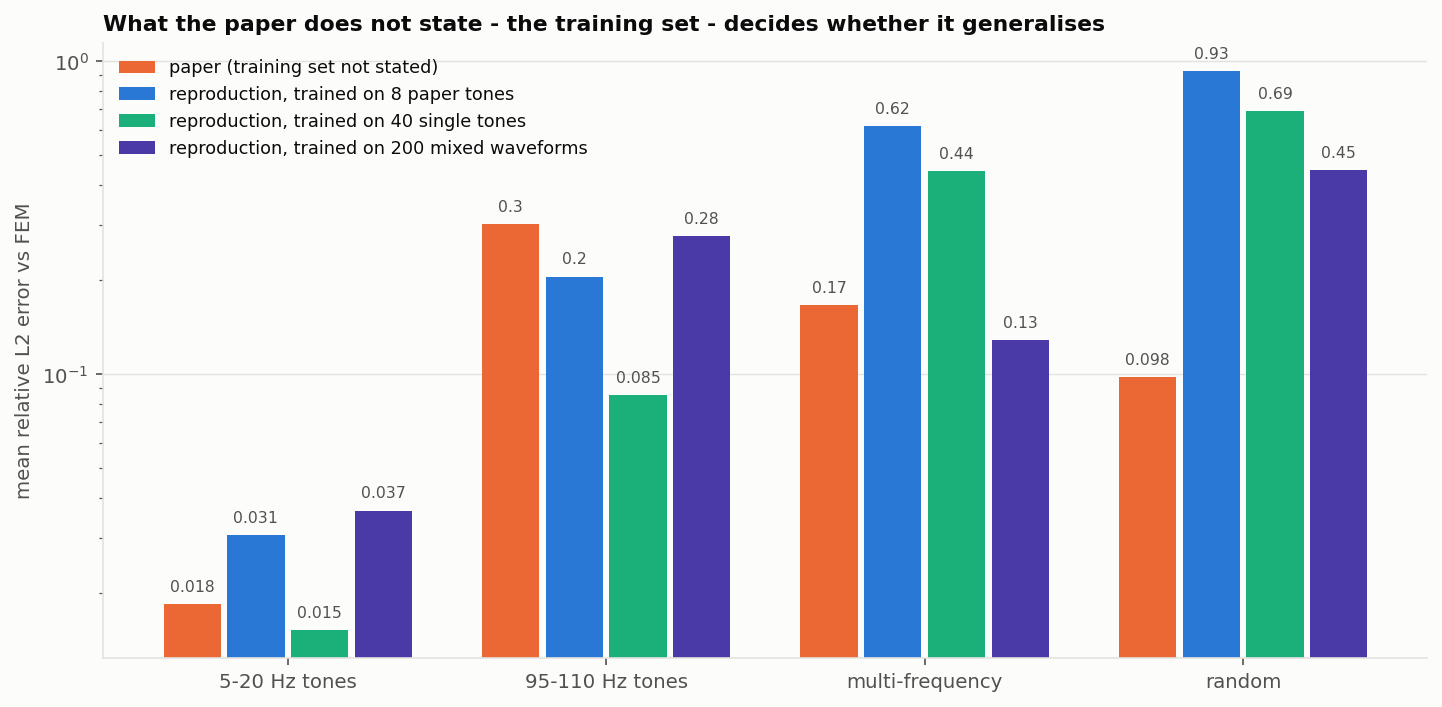
\includegraphics[width=0.7\linewidth]{figures/ch14r/fr_train.png}
\caption{Mean error by load class for three training sets and the publication's values. Plot of the reproduction report.}\label{fig:vf-fr-train}
\end{figure}

\begin{table}[tbp]
\centering\footnotesize
\caption{Three seeds of the default configuration.}\label{tab:vf-fr-seed}
\begin{tabular}{@{}rrrrr@{}}
\toprule
Seed & 5--20 Hz & 95--110 Hz & Multi-frequency & Random\\
\midrule
0 & $1.51\times10^{-2}$ & $8.53\times10^{-2}$ & 0.443 & 0.691\\
1 & $1.56\times10^{-2}$ & $8.38\times10^{-2}$ & 0.215 & 0.699\\
2 & $1.98\times10^{-2}$ & $1.05\times10^{-1}$ & 0.297 & 0.640\\
\bottomrule
\end{tabular}
\end{table}

\begin{figure}[tbp]
\centering
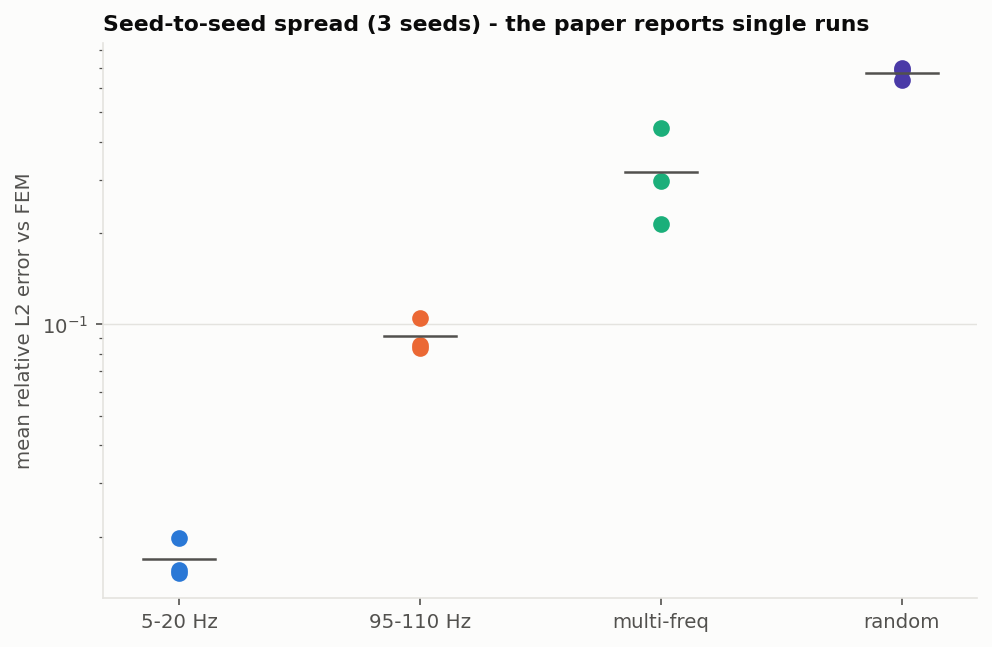
\includegraphics[width=0.7\linewidth]{figures/ch14r/fr_seed.png}
\caption{Three seeds of the default configuration. Plot of the reproduction report.}\label{fig:vf-fr-seed}
\end{figure}

\emph{Is the learned operator linear?} The ROM operator is linear, so its superposition defect is zero; the trained network's mean superposition defect over 12 pairs of tones is $0.632$, and pairs with a tone at 95~Hz or above reach $1.0$--$1.2$. Scaling the 100~Hz waveform in amplitude shows the same (\Cref{tab:vf-fr-lin}, \Cref{fig:vf-fr-lin}): the relative error is $0.0695$ at the trained amplitude and $0.976$ at ten times that amplitude. The network interpolates between trained waveforms and amplitudes and has not learned the linearity of the structure, which is why waveform and amplitude generalisation depend on the training set.

\begin{table}[tbp]
\centering\footnotesize
\caption{Relative error of the 100~Hz tone for scaled amplitude (network trained at 10~N).}\label{tab:vf-fr-lin}
\begin{tabular}{@{}rrrrrr@{}}
\toprule
Amplitude factor & 0.01 & 0.1 & 1 & 10 & 100\\
\midrule
Relative error & 53.1 & 4.84 & 0.0695 & 0.976 & 1.06\\
\bottomrule
\end{tabular}
\end{table}

\begin{figure}[tbp]
\centering
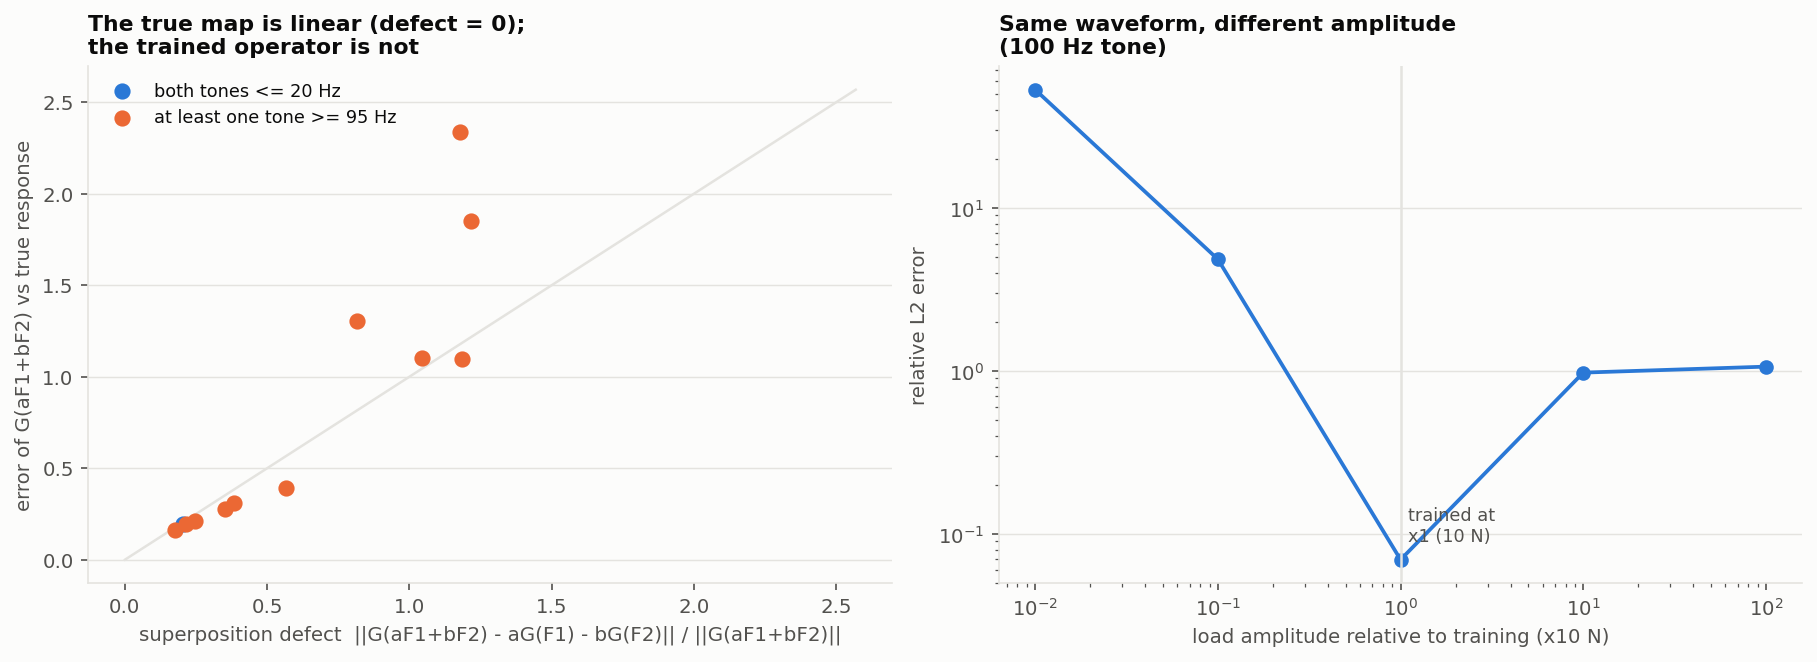
\includegraphics[width=0.9\linewidth]{figures/ch14r/fr_lin.png}
\caption{Left: superposition defect of the trained operator for random pairs of tones. Right: error for the same 100~Hz waveform scaled in amplitude. Plot of the reproduction report.}\label{fig:vf-fr-lin}
\end{figure}

\subsection*{Results: parameter studies}

Every row trains a fresh network (500 epochs) and reports the mean error over load classes on the finer grid; differences below about $30\,\%$ on the in-range columns and a factor of two on the generalisation columns are within seed noise.

\emph{Physics weight.} \Cref{tab:vf-fr-lambda} and \Cref{fig:vf-fr-lambda}: the best in-range errors occur at small $\lambda$ ($10^{-6}$ to $10^{-3}$) and from $10^{-2}$ upward the 5--20~Hz error rises from $1.5\times10^{-2}$ to $2.6\times10^{-2}$. A data-only network ($\lambda=0$) is $3\,\%$ worse at 5--20~Hz and $21\,\%$ worse at 95--110~Hz than the default, both inside seed noise. With labels from the exact ROM the ROM residual is the same error re-weighted by the dynamic-stiffness operator and so carries no new information.

\begin{table}[tbp]
\centering\footnotesize
\caption{Effect of the physics weight $\lambda$.}\label{tab:vf-fr-lambda}
\begin{tabular}{@{}lrrrrrr@{}}
\toprule
$\lambda$ & 5--20 Hz & 95--110 Hz & Multi-frequency & Random & Final data loss & Final ROM loss\\
\midrule
0 (data only) & $1.56\times10^{-2}$ & $1.03\times10^{-1}$ & 0.37 & 0.66 & $4.3\times10^{-4}$ & ---\\
$10^{-6}$ & $1.53\times10^{-2}$ & $9.97\times10^{-2}$ & 0.369 & 0.66 & $4.2\times10^{-4}$ & $1.2$\\
$10^{-4}$ & $1.46\times10^{-2}$ & $8.62\times10^{-2}$ & 0.384 & 0.651 & $3.2\times10^{-4}$ & $1.3\times10^{-1}$\\
$10^{-3}$ (default) & $1.52\times10^{-2}$ & $8.53\times10^{-2}$ & 0.443 & 0.691 & $2.8\times10^{-4}$ & $3.7\times10^{-2}$\\
$10^{-2}$ & $2.22\times10^{-2}$ & $9.60\times10^{-2}$ & 0.368 & 0.781 & $4.2\times10^{-4}$ & $1.9\times10^{-2}$\\
$10^{-1}$ & $2.47\times10^{-2}$ & $8.54\times10^{-2}$ & 0.509 & 0.82 & $5.2\times10^{-4}$ & $7.8\times10^{-3}$\\
1 & $2.62\times10^{-2}$ & $1.44\times10^{-1}$ & 0.34 & 0.746 & $2.0\times10^{-3}$ & $2.5\times10^{-3}$\\
\bottomrule
\end{tabular}
\end{table}

\begin{figure}[tbp]
\centering
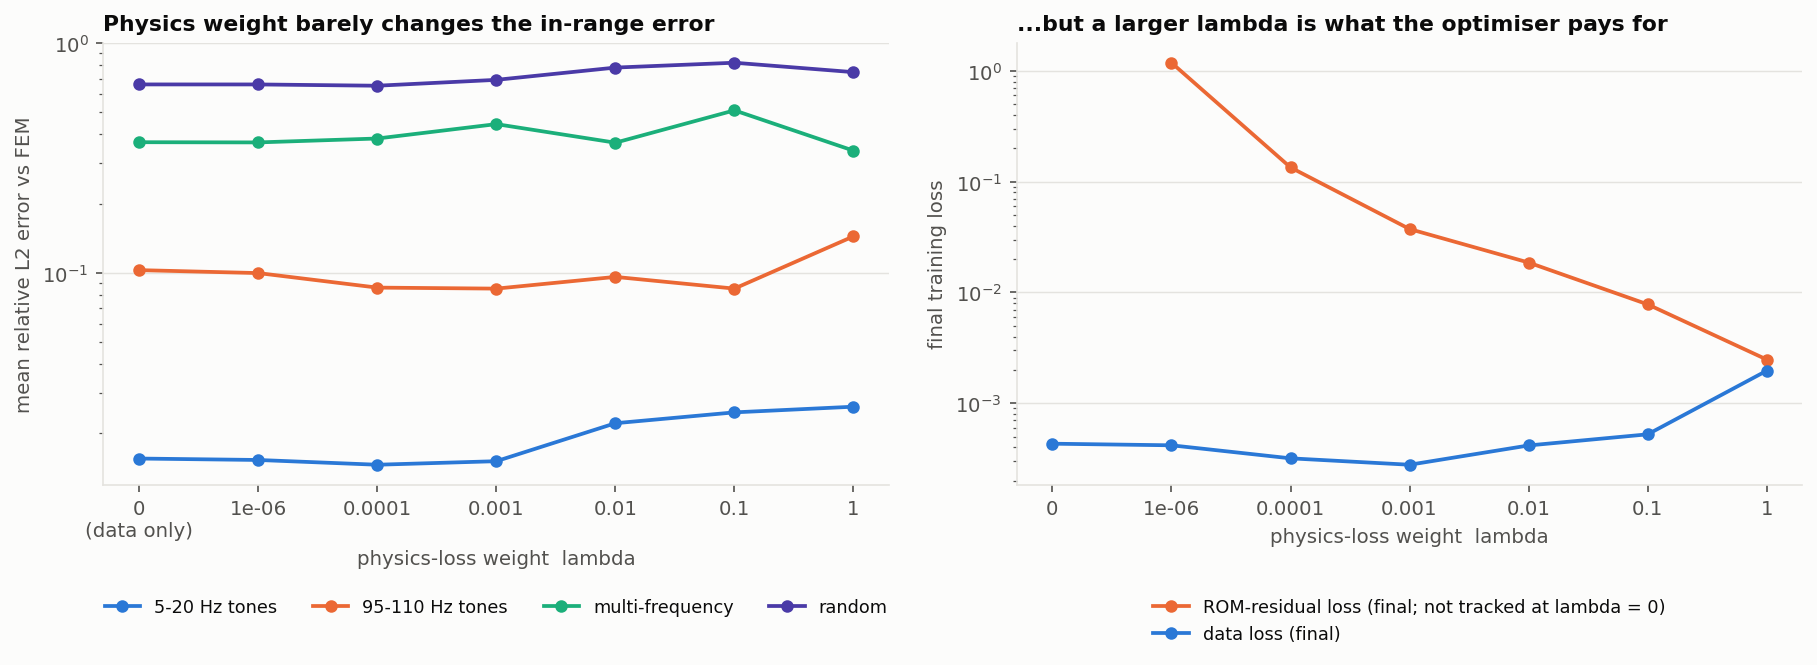
\includegraphics[width=0.9\linewidth]{figures/ch14r/fr_lambda.png}
\caption{Error against the physics weight $\lambda$. Plot of the reproduction report.}\label{fig:vf-fr-lambda}
\end{figure}

\emph{Resolution, width and ROM order.} \Cref{tab:vf-fr-hyper} and \Cref{fig:vf-fr-hyper}: error falls up to 256--512 points per excitation and then stops improving while training time keeps rising (the publication's 6.25\,\% is on the knee); width 128 matches width 256 at $38\,\%$ of the training time; and the ROM order does not change accuracy, as the publication finds, but unlike its $1.1\times10^{3}$, $5.8\times10^{3}$, $1.6\times10^{4}$~s the training time is flat here because the cost is dominated by the width-256 Fourier layers and not by the number of reduced channels. The first-order forward difference that an analysis predicted to carry a 0.25~rad phase error at 100~Hz does not change the result at $\lambda=10^{-3}$, where the data loss dominates, and row scaling of the residual by $\operatorname{diag}(\mathbf K)$ makes the in-range error about $45\,\%$ worse by raising the effective weight of the physics term.

\begin{table}[tbp]
\centering\footnotesize
\caption{Resolution, width and ROM order (mean errors on the finer grid).}\label{tab:vf-fr-hyper}
\begin{tabular}{@{}llrrrr@{}}
\toprule
Parameter & Value & 5--20 Hz & 95--110 Hz & Multi-frequency & Train time (s)\\
\midrule
Points per excitation & 64 & $8.03\times10^{-2}$ & 1.24 & 0.469 & 68\\
 & 128 & $2.80\times10^{-2}$ & $2.15\times10^{-1}$ & 0.347 & 84\\
 & 256 & $1.72\times10^{-2}$ & $9.31\times10^{-2}$ & 0.367 & 102\\
 & 512 & $1.52\times10^{-2}$ & $8.53\times10^{-2}$ & 0.443 & 132\\
 & 1024 & $1.86\times10^{-2}$ & $9.94\times10^{-2}$ & 0.492 & 198\\
 & 2048 & $2.08\times10^{-2}$ & $1.07\times10^{-1}$ & 0.49 & 326\\
\addlinespace
Network width & 16 & $6.24\times10^{-2}$ & $2.38\times10^{-1}$ & 0.892 & 24\\
 & 32 & $3.68\times10^{-2}$ & $1.78\times10^{-1}$ & 0.859 & 22\\
 & 64 & $2.06\times10^{-2}$ & $1.32\times10^{-1}$ & 0.664 & 32\\
 & 128 & $1.34\times10^{-2}$ & $8.99\times10^{-2}$ & 0.477 & 51\\
 & 256 & $1.52\times10^{-2}$ & $8.53\times10^{-2}$ & 0.443 & 133\\
\addlinespace
ROM order & 3 & $1.52\times10^{-2}$ & $8.53\times10^{-2}$ & 0.443 & 133\\
 & 10 & $1.45\times10^{-2}$ & $1.22\times10^{-1}$ & 0.448 & 136\\
 & 20 & $2.39\times10^{-2}$ & $1.41\times10^{-1}$ & 0.438 & 139\\
\bottomrule
\end{tabular}
\end{table}

\begin{figure}[tbp]
\centering
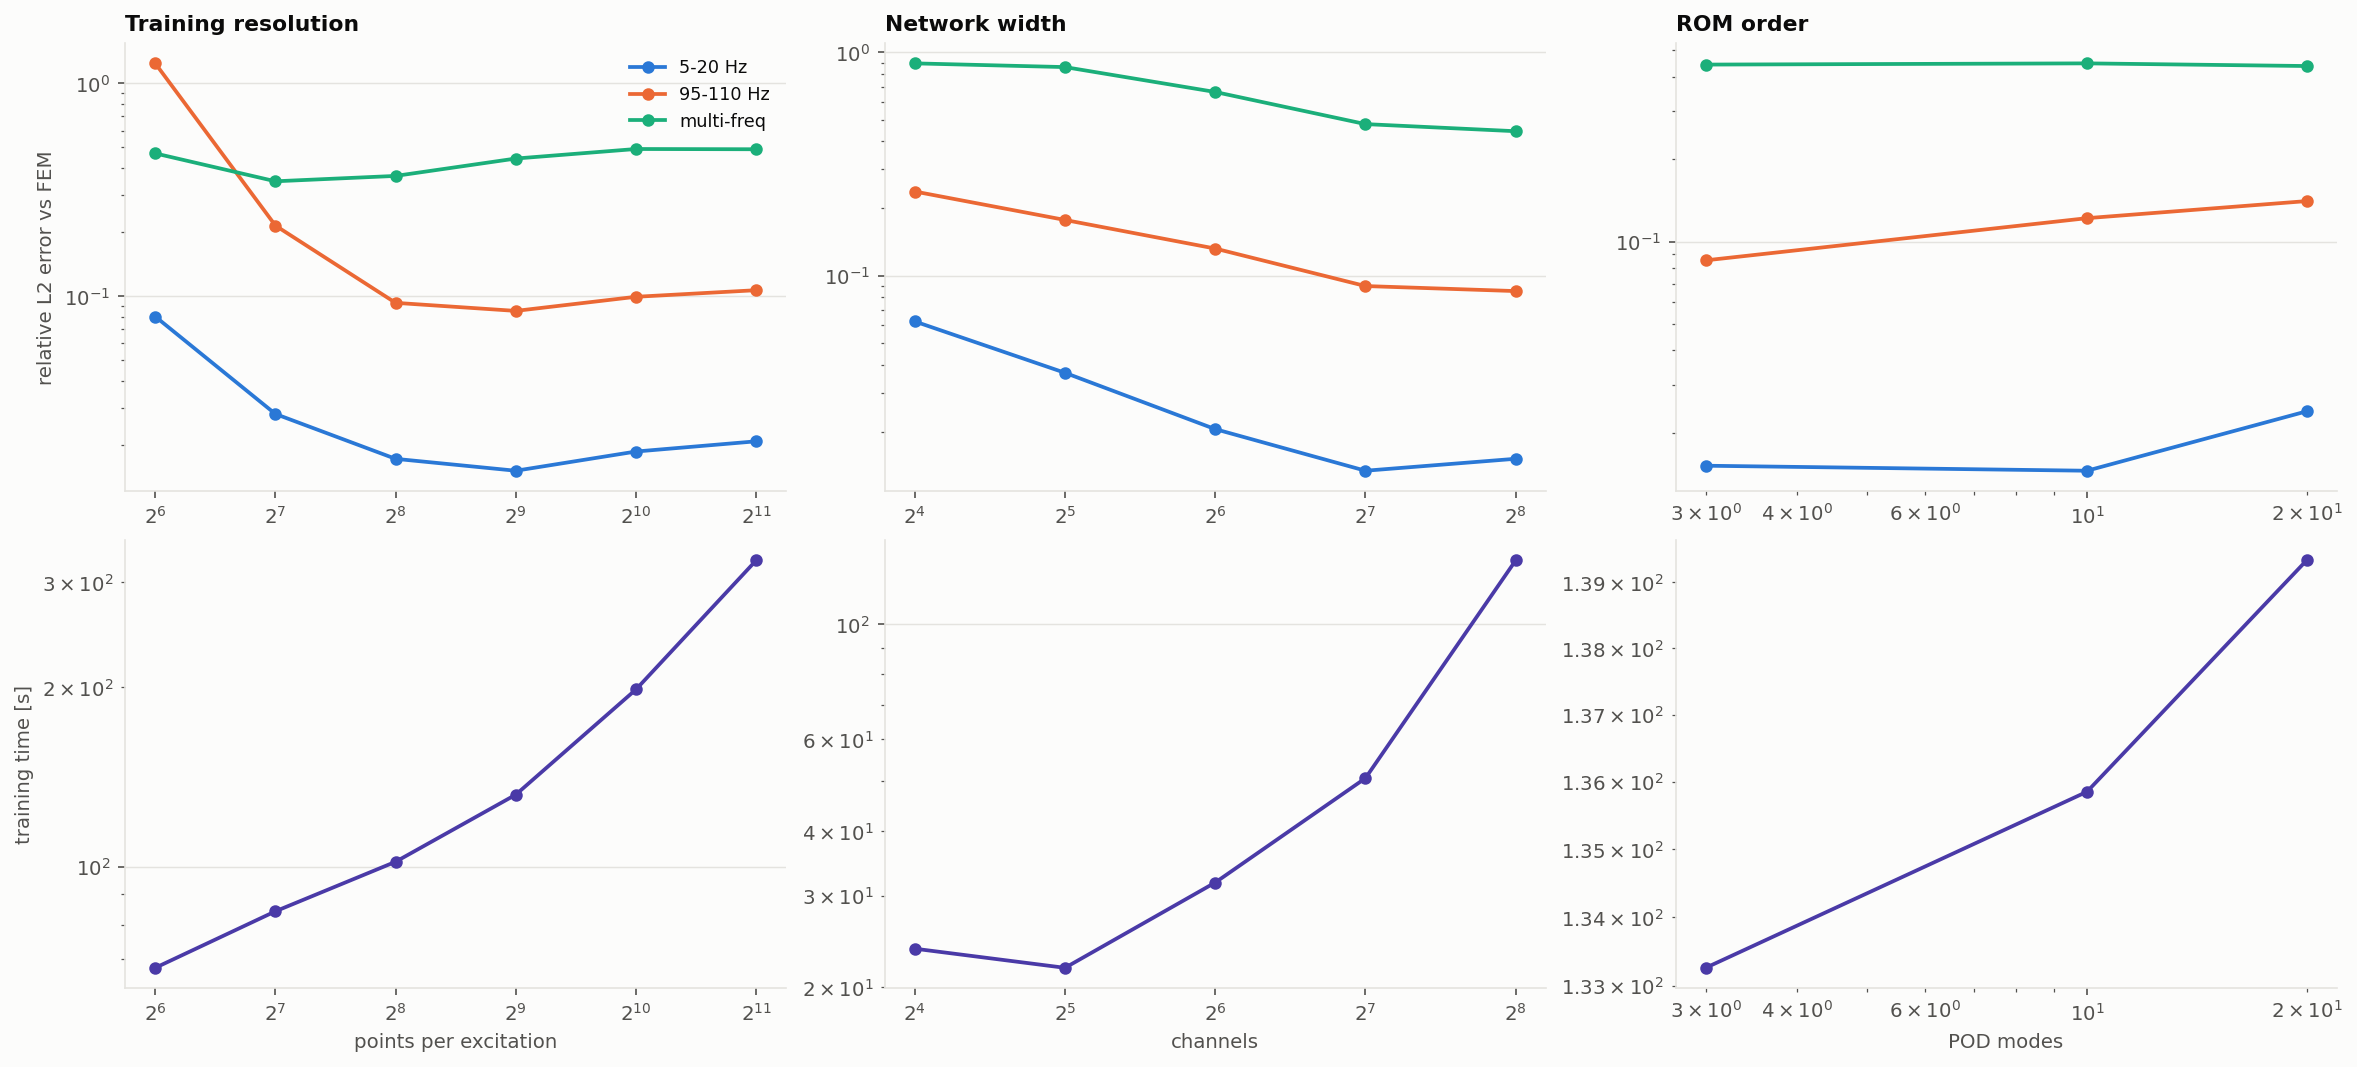
\includegraphics[width=0.98\linewidth]{figures/ch14r/fr_hyper.png}
\caption{Error and training time against the training resolution, the network width and the ROM order. Plot of the reproduction report.}\label{fig:vf-fr-hyper}
\end{figure}

\subsection*{Results: PINN baselines and cost}

The publication gives no architecture, collocation set or budget for its PINN, so the baselines are the author's designs. The first attempt (1500 iterations) uses soft initial conditions, equal fixed loss weights, 500 fixed collocation points, random Fourier features with $\sigma=40$ and an output scale of 5 times the static deflection. The tuned version (3000 iterations) uses hard initial conditions $q=q_st^2N(t)$, 2048 resampled collocation points, gradient-norm loss balancing, a Fourier-feature scale $\sigma=f_{\rm exc}T/2$, an output scale from linear vibration theory, forward-mode differentiation and an L-BFGS polish; variants with labels use the ROM solution at the 6.25\,\% training points. \Cref{tab:vf-fr-pinn} and \Cref{fig:vf-fr-pinn} give the errors. First-attempt baselines are at about 1.0 (no learning) from 20~Hz upward, with or without labels; tuning gives 3 to 30 times lower error at 5~Hz and makes Fourier features and labels help, but not above 20~Hz without labels; with tuning and labels the best baseline reaches $0.30$--$0.38$ at 20--110~Hz and the operator is $2.7$ to $11$ times more accurate there. The publication's two orders of magnitude over a PINN is reached only against first-attempt PINNs ($38$--$44$ times at 5--20~Hz, 15 times at 100~Hz here); a stronger PINN setup might narrow the gap, and each configuration is one run.

\begin{table}[tbp]
\centering\footnotesize
\caption{Relative $L_2$ error of per-tone PINN baselines against the FEM.}\label{tab:vf-fr-pinn}
\begin{tabular}{@{}llrrrrr@{}}
\toprule
Tone & Setup & PINN & FF-PINN & PINN + data & FF-PINN + data & Operator\\
\midrule
5 Hz & first attempt & 0.446 & 0.999 & 0.433 & 0.999 & ---\\
5 Hz & tuned & 0.136 & 0.0457 & 0.0604 & 0.0298 & 0.0101\\
20 Hz & first attempt & 0.991 & 0.997 & 0.991 & 0.997 & ---\\
20 Hz & tuned & 1.17 & 0.793 & 0.923 & 0.297 & 0.0262\\
100 Hz & first attempt & 1.01 & 1.01 & 1.01 & 1.01 & ---\\
100 Hz & tuned & 1.01 & 0.897 & 0.575 & 0.38 & 0.0657\\
110 Hz & first attempt & 0.996 & 0.983 & 0.995 & 0.982 & ---\\
110 Hz & tuned & 0.985 & 0.92 & 0.567 & 0.38 & 0.143\\
\bottomrule
\end{tabular}
\end{table}

\begin{figure}[tbp]
\centering
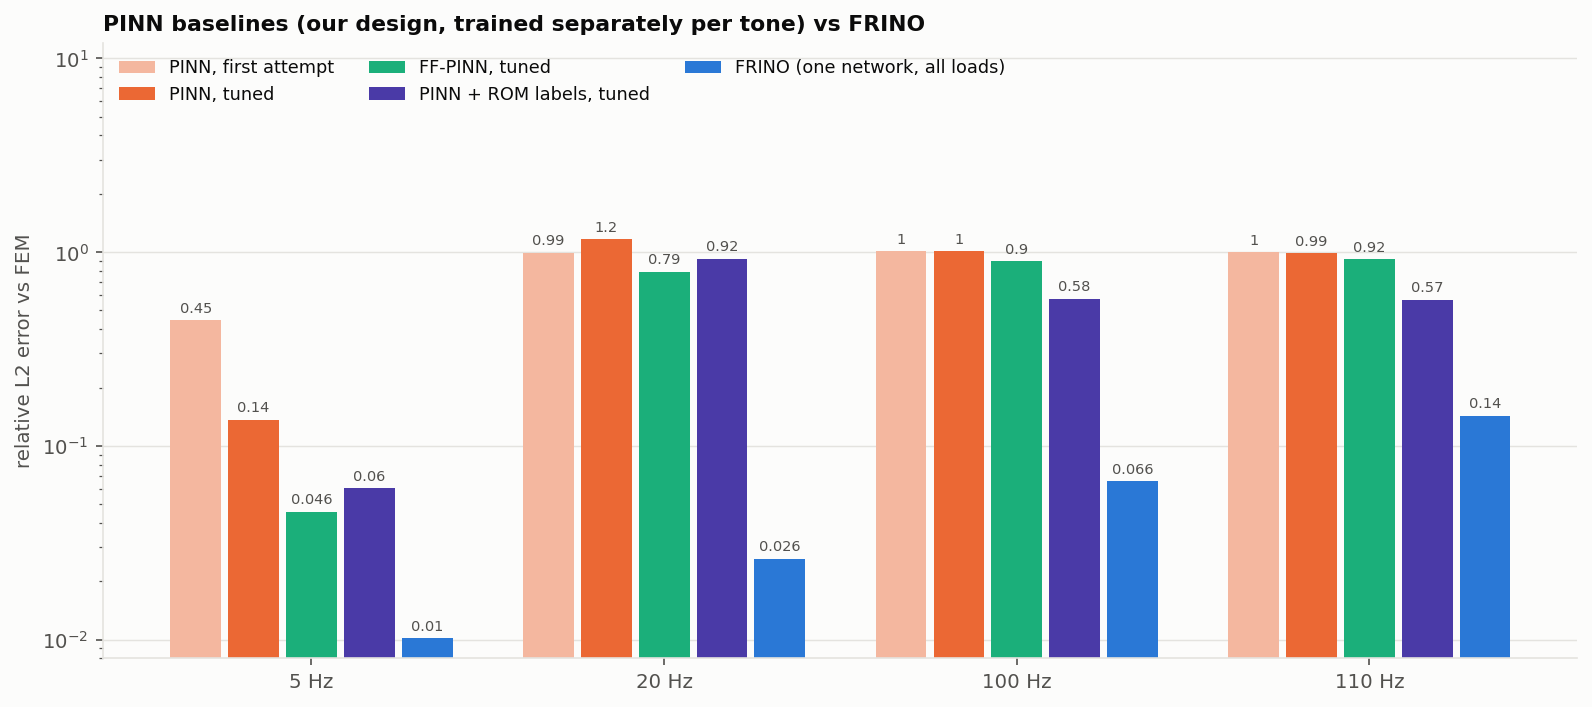
\includegraphics[width=0.9\linewidth]{figures/ch14r/fr_pinn.png}
\caption{Per-tone PINN baselines against the operator. Plot of the reproduction report.}\label{fig:vf-fr-pinn}
\end{figure}

\emph{Cost.} \Cref{tab:vf-fr-cost} and \Cref{fig:vf-fr-cost}: for this linear benchmark the exact frequency-domain solution of the publication's Eq.~(20) costs $18.1$~ms, the same order as the operator's inference ($11$~ms), so its $139$~s of training is never repaid against it (break-even about $2\times10^{4}$ loads); against the CPU full-order solve the break-even is about 3 loads, and against ROM time stepping about 16 (overstated, since that GPU time stepping is launch-bound and a CPU loop is faster). A fair speed claim for this linear problem must compare with the frequency-domain solve; the 4580~s of finite element time in the publication's Table~2 is about 100 times slower than the solve here, which inflates its ratio.

\begin{table}[tbp]
\centering\footnotesize
\caption{Seconds per excitation on the study machine.}\label{tab:vf-fr-cost}
\begin{tabular}{@{}lr@{}}
\toprule
Method & Time per excitation\\
\midrule
FOM Newmark, CPU SuperLU (4032 free dofs, 8192 steps; extrapolated from 300 steps) & 47.0 s\\
FOM Newmark, GPU, batch of 12 (per load) & 17.2 s\\
ROM Newmark (3 modes, GPU; kernel-launch bound) & 8.45 s\\
ROM exact frequency-domain solve, Eq.~(20) (GPU) & 18.1 ms\\
Operator inference (512 points, GPU) & 11.0 ms\\
Operator training (once) & 139 s\\
\bottomrule
\end{tabular}
\end{table}

\begin{figure}[tbp]
\centering
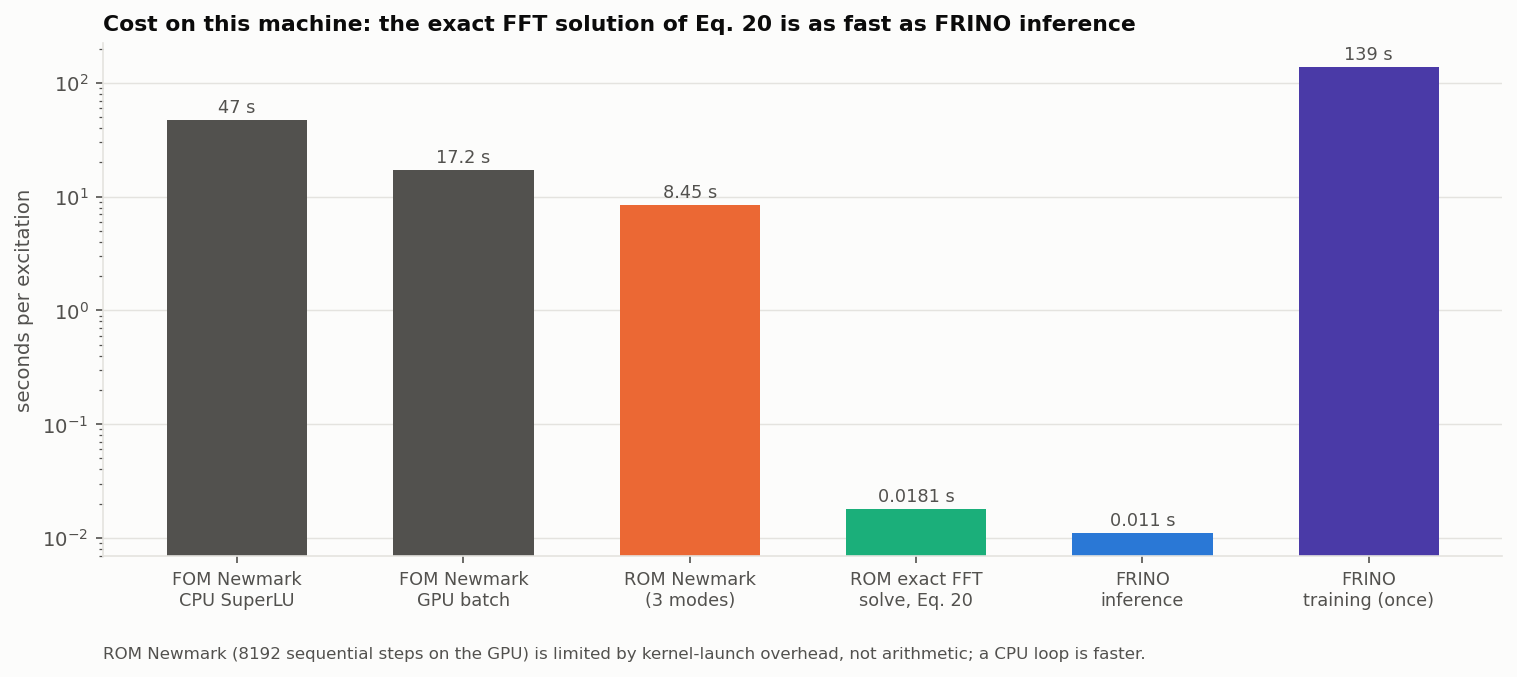
\includegraphics[width=0.7\linewidth]{figures/ch14r/fr_cost.png}
\caption{Seconds per excitation on the study machine. Plot of the reproduction report.}\label{fig:vf-fr-cost}
\end{figure}

\begin{figure}[tbp]
\centering
\includegraphics[width=0.7\linewidth]{figures/ch14_frino.pdf}
\caption{Neural operator of \citet{yang2025frino}: mean relative error for single tones at low and high frequency, multi-frequency loads and random loads, for three training sets. Dashed lines are the publication's values. With 40 tones the multi-frequency and random errors are \cvfFrinoMulti{} and \cvfFrinoRandom. Redrawn by \texttt{scripts/ch14\_assets.py} from the saved outputs of the study; the study itself was not re-run for this book.}\label{fig:vf-frino}
\end{figure}

\subsection*{Comparison with the publication}

\begin{table}[tbp]
\centering\footnotesize
\caption{Claims of \citet{yang2025frino} and the outcome of the reproduction.}\label{tab:vf-fr-cmp}
\begin{tabularx}{\linewidth}{@{}>{\raggedright\arraybackslash}p{4.2cm} >{\raggedright\arraybackslash}X >{\raggedright\arraybackslash}p{2.5cm}@{}}
\toprule
Claim & This work & Outcome\\
\midrule
Accurate low-frequency single tones ($\sim10^{-2}$) & $1.5\times10^{-2}$ mean over 5--20 Hz & reproduced\\
High-frequency errors $\sim0.3$ & $8.5\times10^{-2}$ over 95--110 Hz; the 0.3 equals the error of not learning the forced response & not matched (lower)\\
Multi-frequency and random loads without retraining (0.10--0.20) & 0.443 and 0.691 with 40 tones; best 0.128 and 0.447 with 200 waveforms & not reproduced\\
Learns the natural-frequency content & spectral-peak error at $f_1\le0.115$ & reproduced (in-range tones)\\
Up to 100$\times$ more accurate than a PINN & $37.9\times$ against a first-attempt PINN at 20 Hz; $2.66$--$11.4\times$ against tuned & only against a weak PINN\\
Up to 1000$\times$ faster than a PINN & both milliseconds at inference; a PINN is retrained per load & not meaningful as stated\\
$10^6\times$ faster than FEM & $4265\times$ against the CPU full-order solve (47 s; publication's 4580 s) & partly\\
Zero-shot super-resolution; 6.25\,\% data enough & 16$\times$ finer grid changes tone errors by $<2\times$; plateau from 256--512 points & reproduced\\
$\lambda\le10^{-2}$ appropriate & consistent, but the term has little effect & consistent\\
Width 128--256 optimal; wider overfits & plateau reproduced; no width $>256$ run & overfitting untested\\
Higher ROM order costs more training time & accuracy claim reproduced; training time flat & time claim not\\
\bottomrule
\end{tabularx}
\end{table}

\subsection*{What was not reproduced, and why}

The ANSYS model, the publication's training set and its code are unavailable, so exact numbers cannot be matched; every unstated choice is in \Cref{tab:vf-fr-setup}. Each configuration was trained once except for the three seeds, and differences below the seed spread are not significant. The operator was trained in single precision on a 3~GB GPU; a double-precision run with the package's own FNO blocks is supported but was not run. The PINN baselines are the author's designs, and no width above 256 was run, so the publication's overfitting-with-width claim is untested. An analysis written before the runs made predictions that the outcomes confirmed (consistent units give 345~Hz against $10.9$~Hz as printed; $\zeta_1=2.8\,\%$ against the estimated $2.6\,\%$; the exact frequency-domain solve costs $18$~ms against $11$~ms; the publication's $30\,\%$ high-frequency error equals the forced-part floor; the superposition defect is $0.63$) or contradicted (scale-free residual rows did not help; the estimated third-mode frequency of 175~Hz is 227.8~Hz in the three-dimensional ROM; the forward-difference effect is not visible in the final accuracy).
